\documentclass[a4paper,12pt]{article}

%% Language and font encodings
\usepackage[english]{babel}
\usepackage[utf8x]{inputenc}
\usepackage[T1]{fontenc}

%% Sets page size and margins
\usepackage[a4paper,top=3cm,bottom=2cm,left=3cm,right=3cm,marginparwidth=1.75cm]{geometry}

%% Useful packages
\usepackage{amsmath}
\usepackage{graphicx}
% \usepackage[colorinlistoftodos]{todonotes}
% \usepackage[colorlinks=true, allcolors=blue]{hyperref}

\usepackage{tikz}

\newcommand{\aj}{The Astronomical Journal}
\newcommand{\apj}{The Astrophysical Journal}
\newcommand{\nat}{Nature}

\begin{document}

\title{Binaries}
\author{Pedro Lacerda}

\maketitle

\begin{abstract}
A large fraction of Kuiper belt objects are binary. Binaries are especially prevalent among the cold classical population, which consists of objects in low inclination, nearly circular orbits between 40 and 45 AU.  The current low number density and high velocity dispersion in the Kuiper belt is not conducive to binary formation, so most pairs are believed to have formed at an earlier time, when the belt was more densely populated and dynamically colder.  Focussing on the time window when binaries formed, we investigate how the efficiencies of binary formation and destruction impact the resulting binary fraction.
\end{abstract}

\section{Introduction}

Binaries are common in the Kuiper belt (KB). Typically, KB binaries tend to have comparable mass components and span a wide range of separations, from about 20,000 km down to the limit of spatial resolution.

Binaries are particularly abundant among the cold classical Kuiper belt objects (KBOs), a population believed to best represent the original population formed at KB distances \cite{2010ApJ...722L.204Parker,2018Icar..306..319Gomes}.

A number of binary formation mechanisms have been proposed: L3 \cite{2002Natur.420..643G}, L2s \cite{2002Natur.420..643G}, two-step process of a moonlet forming collision onto the primary followed by gravitational exchange for a larger secondary companion \cite{2004Natur.427..518F}.

Following the dense phase when most binaries have formed, their abundance has likely slowly but steadily decreased over time.  The binary fractions we estimate in this paper aresafa

We forgo the details of the physics of binary formation and destruction and simply assign probabilities to the processes of binary formation and destruction.

In sections \ref{sec:encounterRate} and \ref{sec:probabilisticModel} we estimate the rate of encounters between KBOs and describe a model to simulate their outcome and the evolution of the binary fraction. In sections \ref{sec:results} and \ref{sec:discussion} we present and discuss our results, and conclude in section \ref{sec:conclusions}.

\section{Encounter Rate}
\label{sec:encounterRate}

In this section we estimate how many encounters will occur between objects in the Kuiper belt. We restrict ourselves to the cold classical region, roughly defined here as a toroid with rectangular section between 40 and 45 AU from the sun, with a height defined by orbital inclination $<5$ deg. The volume of this box is then
\begin{equation}
V_{KB} = 2\pi\times 42.5\,\text{AU}\times 5\,\text{AU} \times 2\tan{(5\deg)}\times 42.5\,\text{AU}\approx 10^4 \,\text{AU}^3
\end{equation}
We assume that the number of objects in the region prior to the mass removal events was $N_{KBO}=1.5\times 10^5$, which results in a number density of 
\begin{equation}
n =\frac{N_{KBO}}{V_{KB}}=15 \,\text{AU}^{-3}.
\end{equation}
For the encounter cross-section we take a circular area 
\begin{equation}
\sigma =\pi R^2 = \pi  (10^5 \,\text{km})^2=1.4\times 10^{-6} \text{AU}^2
\end{equation}
where $R$ is the semimajor axis of the most widely separated binary known in the cold classical belt, 2001 QW$_{322}$. The velocity dispersion is of order 
\begin{equation}
u=0.5 \,\text{km s}^{-1}=0.1 \,\text{AU yr}^{-1}
\end{equation}
The particle-in-a-box encounter rate for the population is
\begin{equation}
n \sigma u \,N_{KBO} = 0.33 \,\text{yr}^{-1} = 100 \;\text{per orbit}
\end{equation}
where $n\sigma u=0.7\times 10^{-3}$ orbit$^{-1}$ is the encounter rate per KBO.

\begin{table}
\centering
\begin{tabular}{lll}
Quantity & Symbol & Value \\ \hline
number of KBOs & $N_{KBO}$ & $1.5\times10^5$ \\
distance to KB & $r_{KB}$ & $42.5$ AU \\
width of KB & $w_{KB}$ & $5$ AU \\
orbital inclination at KB & $i_{KB}$ & $5$ deg \\
system state & $i$ & \\
number of particles, single or binary & $K$ & \\
\end{tabular}
\end{table}

\section{Probabilistic Model}
\label{sec:probabilisticModel}

We consider a system of $N_\text{KBO}$ objects that can exist as singles or in binaries.  For simplicity we take $N_\text{KBO}$ to be even.  The system can be in one of $n=N_\text{KBO}/2+1$ states, each state, $E_i$, having $B=i$ binaries and $S=N_\text{KBO}-2i$ singles, with $i\in\{0,1,\dots,n-1\}$.  In state $E_i$, the system has $K=N-i$ particles (single or binary), a fraction of singles $s_i=(N-2i)/(N-i)$, and a fraction of binaries $b_i=i/(N-i)$ (see Figs.~\ref{fig:singlesbinaries} and \ref{fig:fractionsinglesbinaries}).

\begin{figure}
\centering
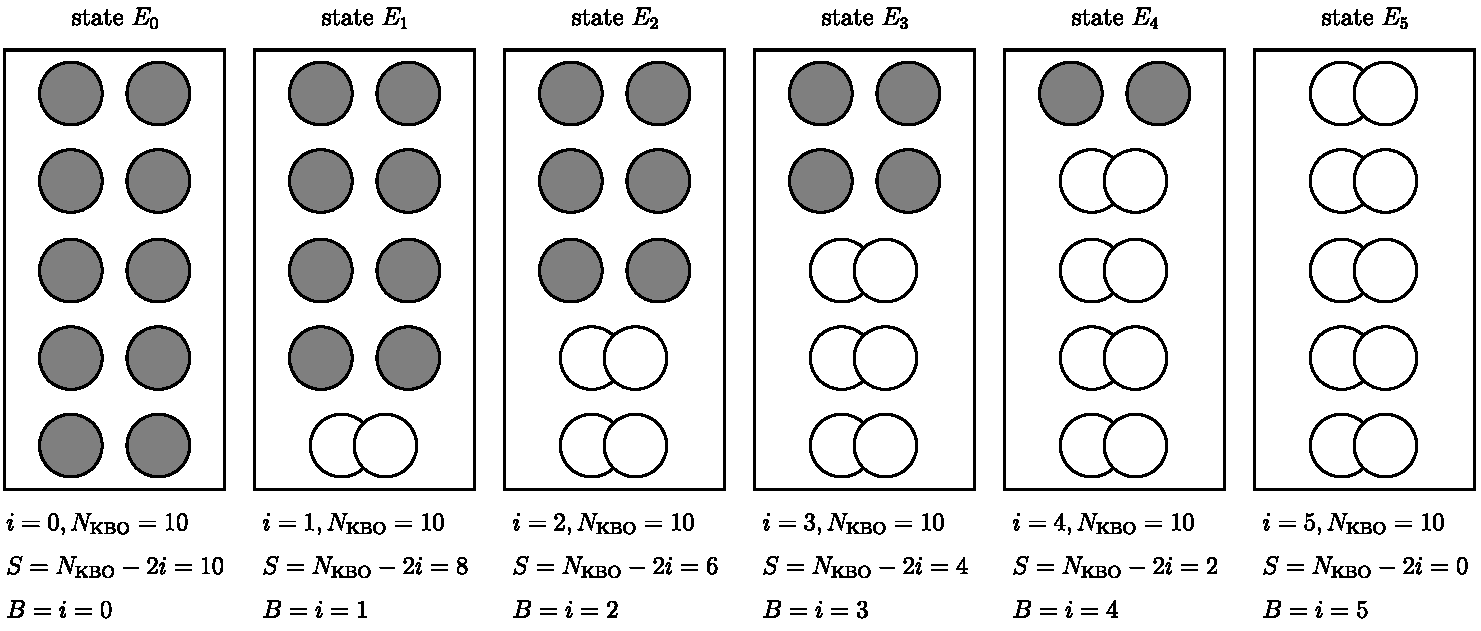
\includegraphics[width=\textwidth]{SinglesBinaries}
\caption{\label{fig:singlesbinaries}
Example of the number of single and binary KBOs in each system state, $E_i$, shown as boxes. In each state, single KBOs are shown as blue disks and binary KBOs as red overlapping disks. In state $E_i$ there are $B=i$ binaries and $S=N_\text{KBO}-2i$ singles.}
\end{figure}

\begin{figure}
\centering
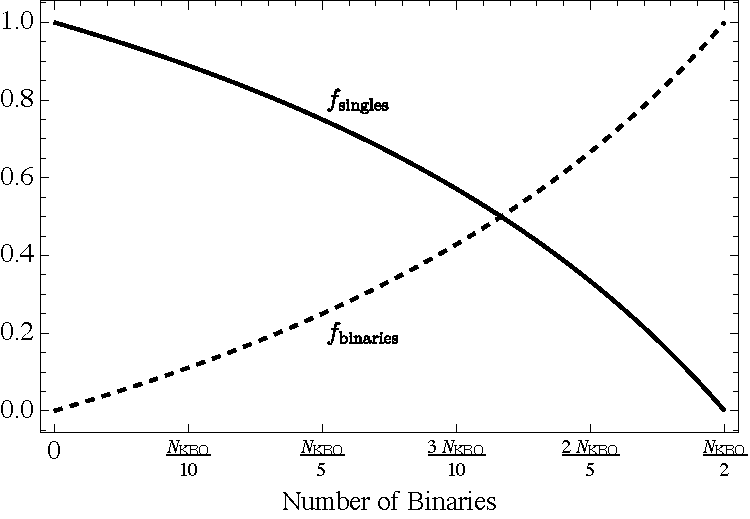
\includegraphics[width=0.7\textwidth]{FractionOfSinglesBinaries}
\caption{\label{fig:fractionsinglesbinaries}
Fractions of single KBOs and binary KBOs in the system as a function of the number of binaries.}
\end{figure}

When two of the $K$ particles encounter each other, they interact. Four types of encounter between particles can occur: a single may meets a single or a binary, and a binary may meet a single or a binary. A single-single encounter may result in a binary being formed (with probability $P_1$), or in simple scattering (with probability $1-P_1$). Single-binary or binary-single encounters may result in survival of the binary (through simple scattering of the single, or exchange of one of the binary components with the single, with combined probability $P_2$) or disruption into three singles ($1-P_2$). Binary-binary encounters may lead to survival of both binaries (through scattering or component exchanges, with combined probability $P_3$) or disruption of one of the binaries into two singles ($1-P_3$). Lower probability scenarios such as formation of triples or double disruption in binary-binary encounters are disregarded.

An encounter between particles can be fully analysed probabilistically following Fig.~\ref{fig:chain_of_probability}. For instance, the probability of drawing a single from the particle ensemble in state $E_i$ is $s_i$, and then the probability that that particle meets another single is also $s_i$ (assuming large $N_\text{KBO}$). If the probability that the two singles end up as a binary following the encounter is $P_1$, then the probability that a binary forms in the system from an encounter between singles is
\begin{equation} \label{eq:P1}
\text{Pr}(E_i\rightarrow E_{i+1}) = s_i^2 P_1.
\end{equation}
\noindent which is the probability that the system moves from state $E_i$ to state $E_{i+1}$.

Similarly for the remaining types of encounters, following an encounter between two of the $K$ particles, the system can move to state $E_{i-1}$ if a binary is disrupted or remain in state $E_i$ if the number of binaries remains the same.  The probability of those state transitions can be assessed by inspection of Fig.~\ref{fig:chain_of_probability}.  In addition to the probability of the transition $E_i\rightarrow E_{i+1}$ in Eq.~\eqref{eq:P1}, the system will move to state $E_{i-1}$ or $E_i$ with probabilities
\begin{align}
\text{Pr}(E_i\rightarrow E_{i-1}) &= 2 s_i b_i (1-P_2) + b_i^2 (1-P_3) \label{eq:E1E0} \\
\text{Pr}(E_i\rightarrow E_i) &= s_i^2 (1-P_1) + 2 s_i b_i P_2 + b_i^2 P_3 \label{eq:E1E1}
\end{align}
where $s_i$ and $b_i$ are the single and binary fractions in state $E_i$, and $P_1$, $P_2$, and $P_3$ are probabilities which depend on the physical processes responsible for binary formation and disruption. $P_1$ can be thought of as a \textit{formation} probability, while $P_2$ and $P_3$ can be seen as \textit{survival} probabilities. It can be shown algebraically from Eqs.\ \eqref{eq:P1}, \eqref{eq:E1E0} and \eqref{eq:E1E1} that
\begin{equation} \label{eq:Ptot}
\text{Pr}(E_i\rightarrow E_{i+1}) + \text{Pr}(E_i\rightarrow E_{i-1}) + \text{Pr}(E_i\rightarrow E_i)=1
\end{equation}

The time evolution of the system can be modelled by calculating the outcome of successive encounters. For each encounter, a random number between drawn from a uniform distribution over the interval $[0,1]$ can be used to decide, using Eq.~\eqref{eq:Ptot}, whether the system will remain in state $E_i$ or transition to state $E_{i-1}$ or $E_{i+1}$. This type of system is a Markov process, specifically a time-homogeneous, Discrete-Time Markov Chain. 

\begin{figure}
\centering
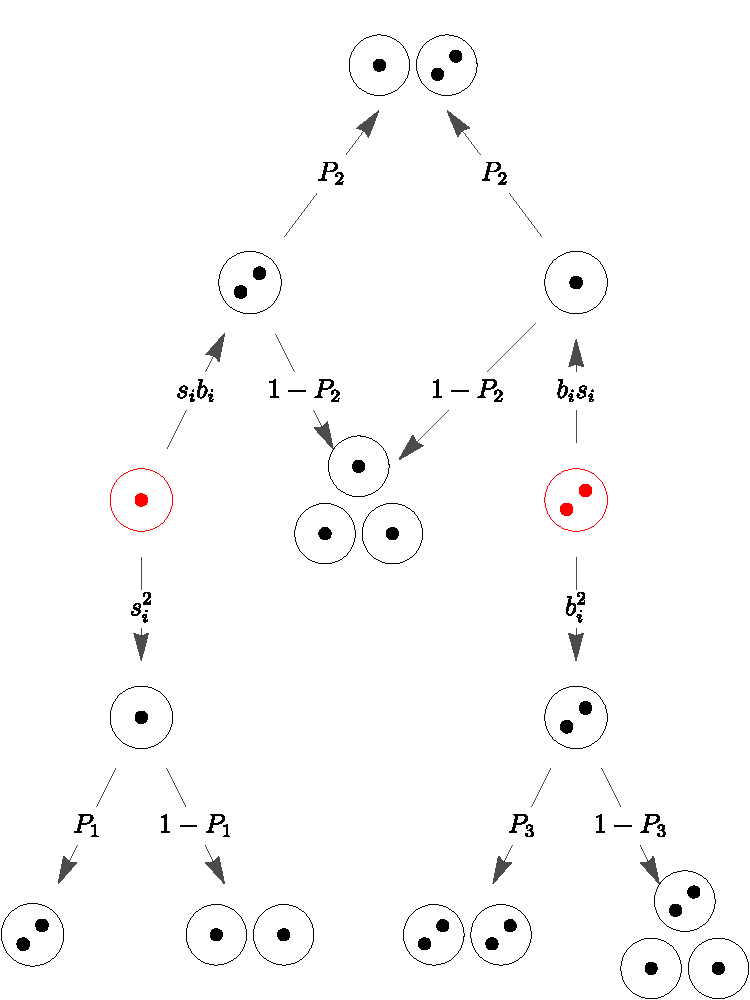
\includegraphics[width=0.5\textwidth]{ProbabilityChain}
\caption{\label{fig:chain_of_probability}
Chain of probability for the outcome of an encounter.  The first step is the choice of the first particle in the encounter (one of the red nodes), which can be single with probability $s_i$ or binary with probability $b_i$.  Hence, in a random encounter, a single object (red single node) may encounter another single with probability $s_i^2$, or a binary with probability $s_i b_i$.  A binary object (red binary node) may encounter a single with probability $b_i s_i$ or another binary with probability $b_i^2$. Single-single encounters lead to the formation of a binary with probability $P_1$ or simply to scattering with probability $1-P_1$.  A binary can survive an encounter with a single with probability $P_2$ or be disrupted with probability $1-P_2$.  Two binaries can scatter of each other and survive with probability $P_3$ or one of the binaries may be disrupted with probability $1-P_3$.  Lower probability scenarios such as formation of triples or double disruption in binary-binary encounters are disregarded.}
\end{figure}

% \begin{equation}
% \left(
% \begin{array}{ccc}
%  s_0^2 \left(1-p_1\right) + 2 s_0 b_0 p_2+b_0^2 p_3 & s_0^2 p_1 & 0 \\
%  2 s_1 b_1 \left(1-p_2\right)+b_1^2 \left(1-p_3\right) & s_1^2 \left(1-p_1\right) + 2 s_1 b_1 p_2+b_1^2 p_3 & s_1^2 p_1 \\
%  0 & 2 s_2 b_2 \left(1-p_2\right)+b_2^2 \left(1-p_3\right) & s_2^2 \left(1-p_1\right) + 2 s_2 b_2 p_2+b_2^2 p_3 \\
% \end{array}
% \right)
% \end{equation}

% \begin{figure}
% 	\centering
% 	\begin{tikzpicture}
%   		\node[draw] (B) at (0,0) {$\{s_0,b_0\}=\{1,0\}$};
% 		\node[draw] (M) at (0,3) {$E_i:\{s_i,b_i\}=\lbrace\frac{N-2i}{N-i},\frac{i}{N-i}\rbrace$};
% 		\node[draw] (E) at (0,6) {$E_i:\{s_{N/2},b_{N/2}\}=\{0,1\}$};
%         \draw[->,>=latex] (M) to (E);
% 		\draw[->,>=latex] (M) to (B);
%         \draw[->,>=latex] (M) to[bend right] (M);
%   	\end{tikzpicture}
%   	\caption{\label{fig:diagram}Do not forget!
%       Make it explicit enough that readers
%           can figure out what you are doing.}
% \end{figure}

\section{Results}
\label{sec:results}

\subsection{Initial binary fraction}
\label{sec:resultInitialBinaryFraction}

We first investigate whether the initial binary fraction matters for our simulations. Traditional models of planetesimal accretion consider that bodies form as singles, which would imply a zero initial binary fraction. But binaries may have formed as a direct consequence of the accretion of KBOs.  The gravitational collapse formation model \cite{2005ApJ...620..459Y,2007Natur.448.1022J} could naturally lead to binary formation, as the angular momentum of the pebble cloud before collapse occurs is too large for a single, fast spinning KBO to form. This path to binary formation has been explored numerically \cite{2010AJ....140..785N} to show that gravitational instability could lead to an initial binary fraction near unity. 

Figure~\ref{fig:doesinitialstatematter} explores the full range of initial binary fractions from 0 to 1 and shows that the binary fraction of the system tends to an equilibrium value that is independent of the initial binary fraction.

\begin{figure}
\centering
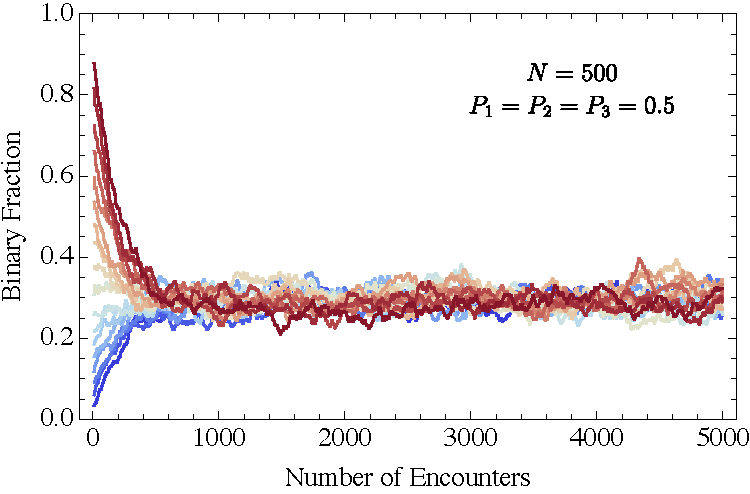
\includegraphics[width=0.7\textwidth]{DoesInitialStateMatter}
\caption{\label{fig:doesinitialstatematter}
Binary fraction reaches an equilibrium value that is independent of the initial binary fraction.}
\end{figure}


\subsection{Timescale to reach equilibrium}
\label{sec:resultTimescaleForEquilibrium}

As the number of KBOs simulated increases so does the possible number of states the system can be in.  Consequently, more encounters may be required to traverse the larger number of states and reach equilibrium. Figure~\ref{fig:doespopulationsizematter} shows that this is indeed the case. The larger the system being considered, the higher the number of encounters needed to reach equilibrium.  

\begin{figure}
\centering
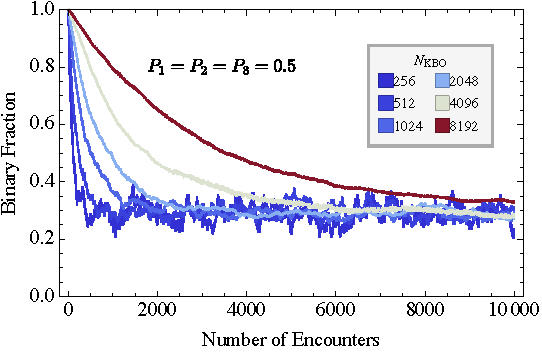
\includegraphics[width=0.7\textwidth]{DoesPopulationSizeMatter}
\caption{\label{fig:doespopulationsizematter}
Binary fraction reaches an equilibrium value faster for smaller $N_\text{KBO}$, but the final fraction is independent of $N_\text{KBO}$.}
\end{figure}

As seen in Fig.~\ref{fig:encountersneededtoreachequilibrium}, which refers to Fig.~\ref{fig:doespopulationsizematter} and plots the number of encounters needed to reach a binary fraction of $0.35$, the number of encounters necessary to reach an equilibrium binary fraction increases linearly with the number of KBOs simulated.  Given our model of the Kuiper belt and our estimated rate of $0.7\times 10^{-3}$ encounters per KBO per orbit, the timescale for the binary fraction to equilibrate would be of order $450$ kyr, which is short compared to the dynamical evolution of the Kuiper belt.

Furthermore, because we consider a fixed volume, the encounter rate increases linearly with the number of particles, as does the number of encounters needed to reach equilibrium.  So, our results are independent of the number of KBOs simulated.  Importantly, the equilibrium binary fraction is independent of the number of KBOs.

In our simulations, once equilibrium is attained, the instantaneous binary fraction will oscillate around the equilibrium value.  The oscillations are visibly larger for smaller systems.  The equilibrium value may be extracted by using a running median over a range of encounters.

\begin{figure}
\centering
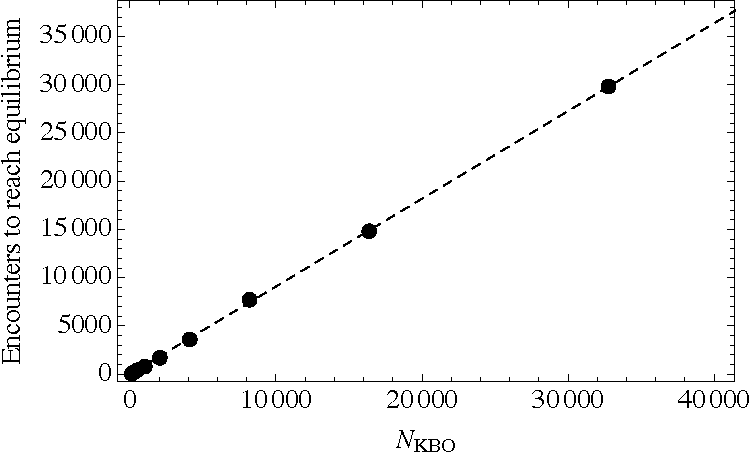
\includegraphics[width=0.7\textwidth]{EncountersNeededToReachEquilibrium}
\caption{\label{fig:encountersneededtoreachequilibrium}
Number of encounters needed to reach the equilibrium binary fraction scales linearly with $N_\text{KBO}$. The dashed line was fit by eye; it goes through the origin and has slope 0.91.}
\end{figure}

\begin{figure}
\centering
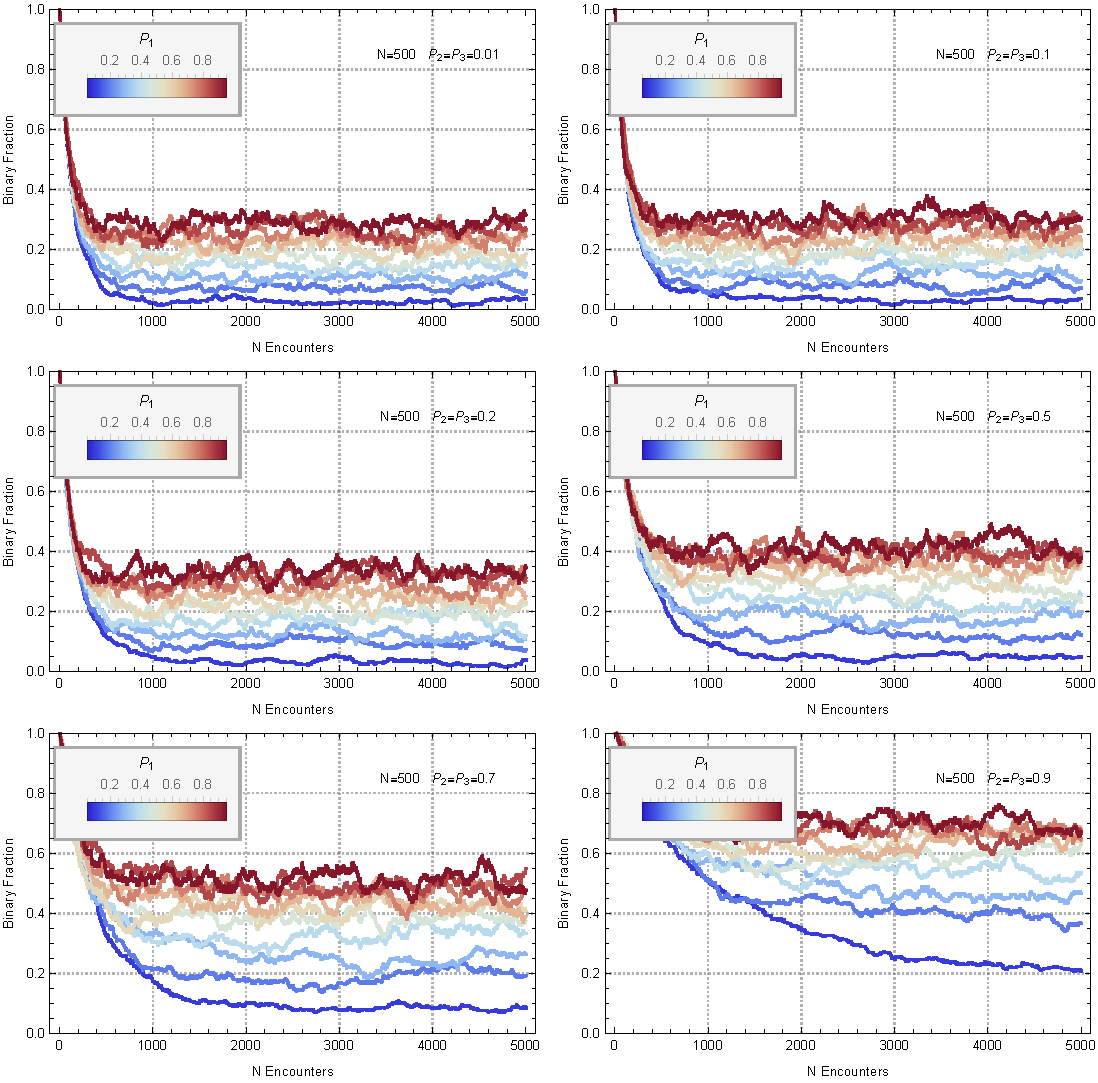
\includegraphics[width=1\textwidth]{P1Matters}
\caption{\label{fig:doesP1matter}
Dependence on $P_1$, the binary formation probability.}
\end{figure}


\section{Subsequent evolution}
\label{sec:SubsequentEvolution}

We focus here on the period where the abundance of binaries varied most dramatically. Beyond this time, we expect the number of binaries to slowly erode over time, as the KB number density declines and encounters velocities approach the current typical 1 km/s. Formation of satellites of large KBOs might still occur (Brown \& Butler, 2018; Canup 2011, McKinnon 2017, Barr \& Schwamb 2016). Therefore, the equilibrium binary fractions we find above should be taken as upper limits.


\bibliographystyle{alpha}
\bibliography{bibliography}

\section{Discussion}
\label{sec:discussion}

\section{Conclusions}
\label{sec:conclusions}

\end{document}